\section{Background}
Understanding the relationship between the depth of the basin, and properties about the resulting modeled delta can be helpful when trying to design numerical experiments.

\section{Model Runs}
Six model runs from Section \ref{sec:standard_model_runs} are used, and an addition 12 model runs in a 10m basin are conducted; 6 of which are run for 5,000 timesteps and the other 6 are run for 10,000 timesteps.
These runs are at ``field-scale" using parameters similar to those from previous studies \cite{Liang2016, Liang2016a}.
This is accomplished by varying the \textit{hB} YAML parameter in the model, the YAML is not included here for brevity, parameters are standard and match those of Section \ref{sec:standard_model_runs}.

\section{Results}
Example final topographies of the three model configurations are provided (Figure \ref{fig:bd_final_topos}), and examples of stratigraphic sections from the standard, 5m deep basin, as well as the 10,000 timestep 10m basin runs are shown (Figures \ref{fig:bd_dips}, \ref{fig:bd_radial}, \ref{fig:bd_horiz}). 

\begin{figure}[!ht]
	\makebox[\textwidth][c]{
	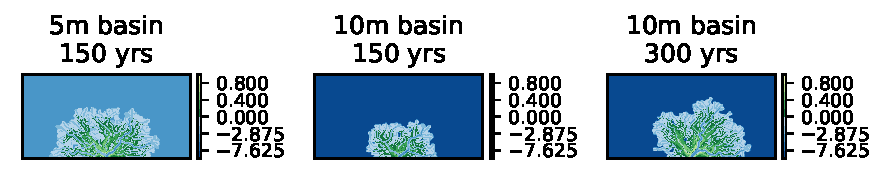
\includegraphics[width=\textwidth]{BasinDepth/figs/final_topos.pdf}
	}	
	\caption{Final topographies for the three scenarios considered.}
	\label{fig:bd_final_topos}
\end{figure}

\begin{figure}[!ht]
	\makebox[\textwidth][c]{
	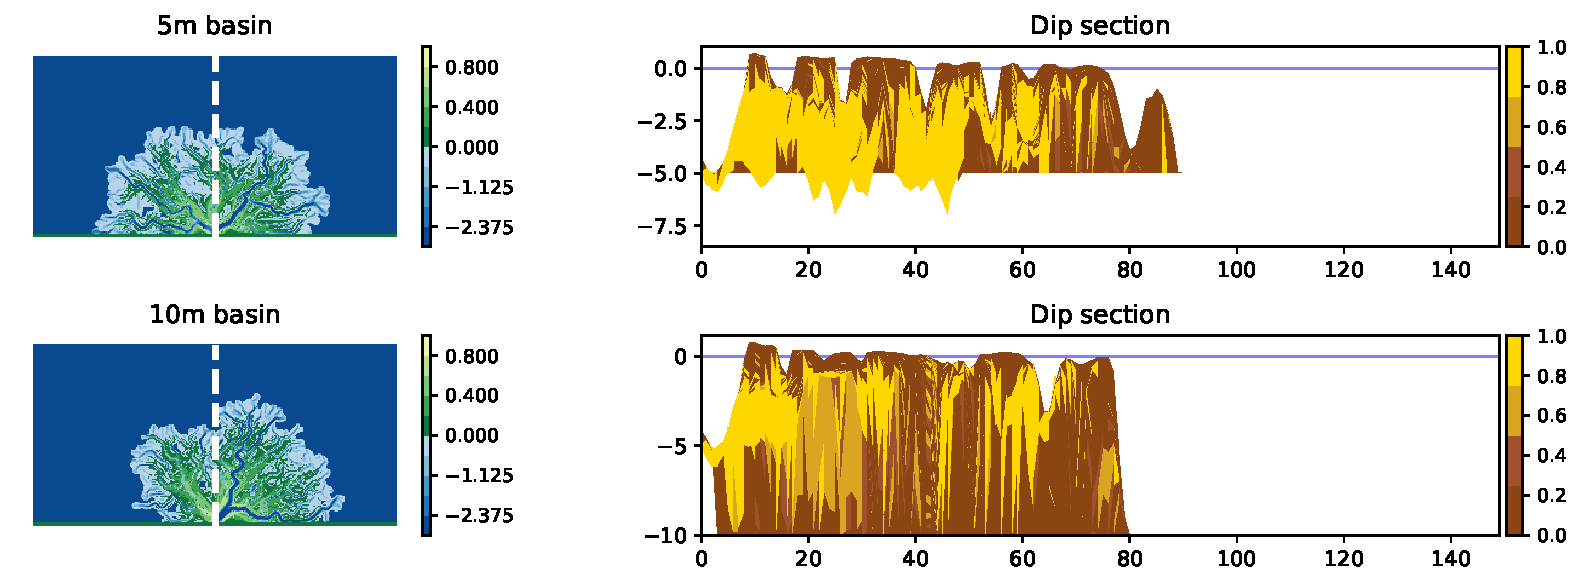
\includegraphics[width=\textwidth]{BasinDepth/figs/demo_dip_sections.pdf}
	}	
	\caption{Demo dip sections taken at the inlet location.}
	\label{fig:bd_dips}
\end{figure}

\begin{figure}[!ht]
	\makebox[\textwidth][c]{
	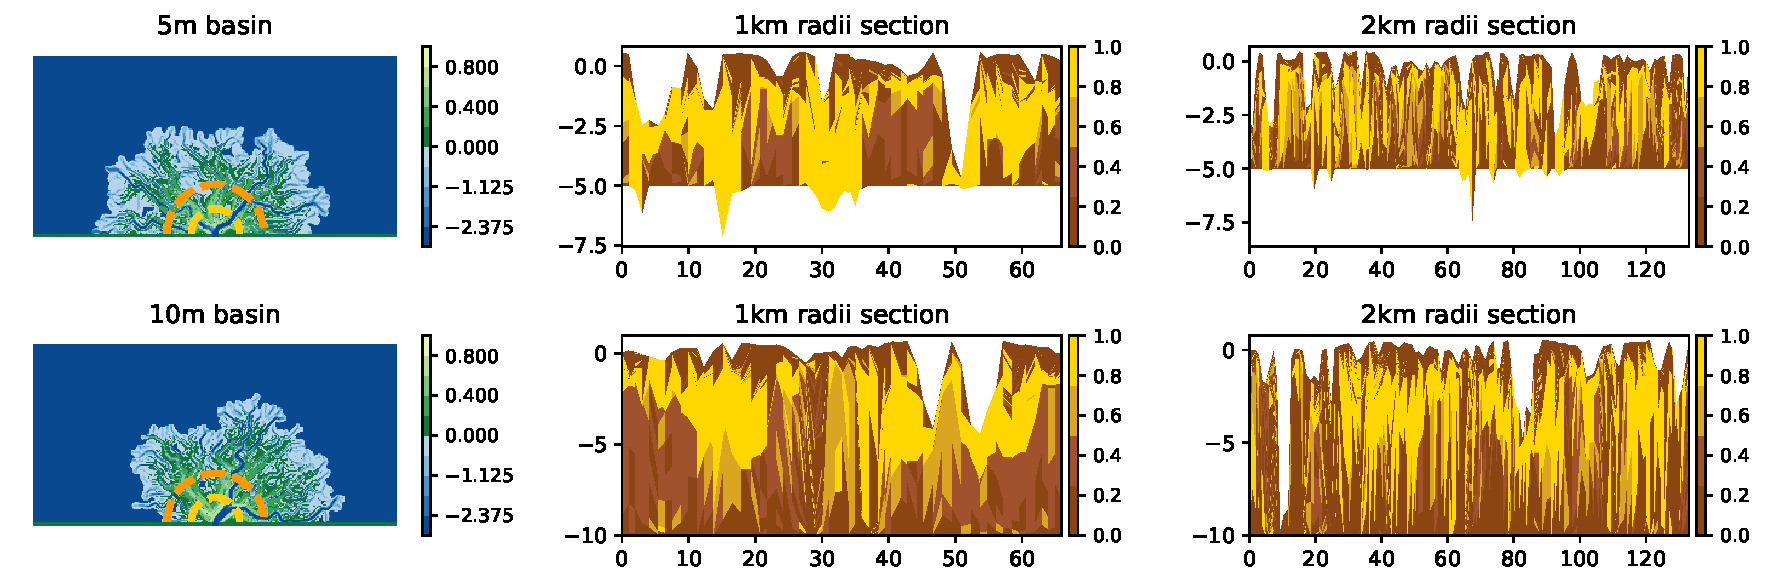
\includegraphics[width=\textwidth]{BasinDepth/figs/demo_radial_sections.pdf}
	}	
	\caption{Demo azimuthal sections taken with radii of 1 and 2km.}
	\label{fig:bd_radial}
\end{figure}

\begin{sidewaysfigure}[!ht]
	\makebox[\textwidth][c]{
	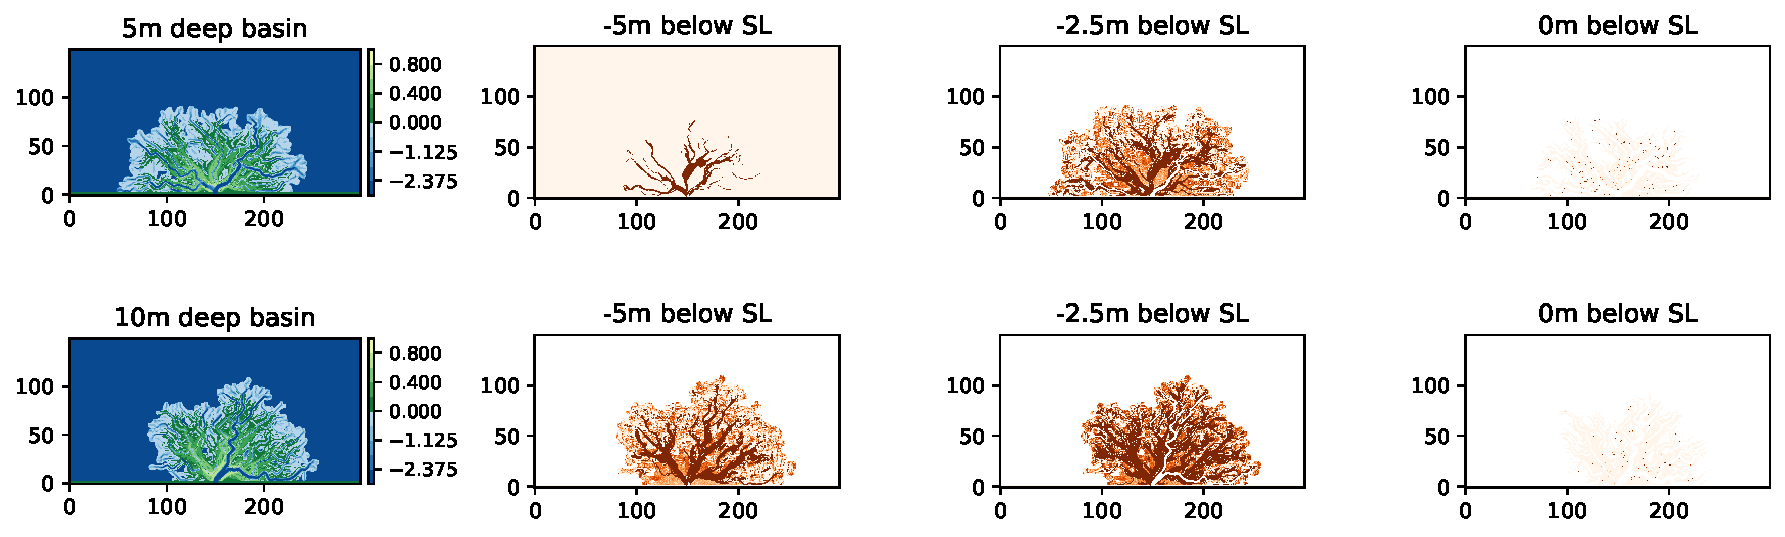
\includegraphics[width=\textwidth]{BasinDepth/figs/demo_horiz_sections.pdf}
	}	
	\caption{Demo horizontal slices of stratigraphy.}
	\label{fig:bd_horiz}
\end{sidewaysfigure}

Several metrics are calculated including the total land area of the modeled deltas (Figure \ref{fig:bd_land_area}), their channelized fractions (Figures \ref{fig:bd_chanfrac_timeseries} \& \ref{fig:bd_chanfrac_box}), and width-to-depth ratios of surface channels along several azimuthal transects with different radii (Figure \ref{fig:bd_wd}).

\begin{figure}[!ht]
	\makebox[\textwidth][c]{
	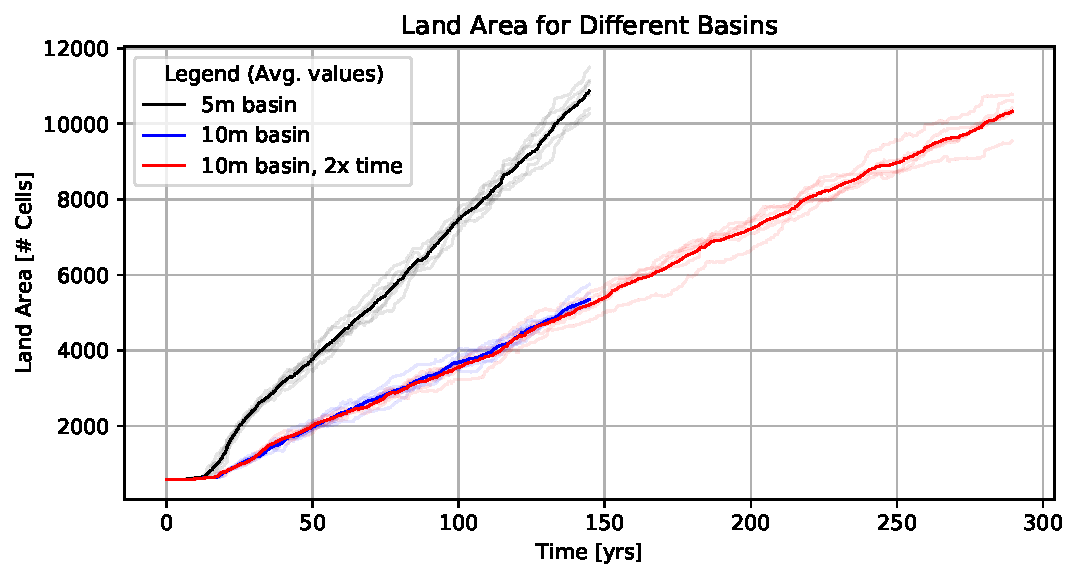
\includegraphics[width=\textwidth]{BasinDepth/figs/basin_land_timeseries.pdf}
	}	
	\caption{Land area timeseries, subaerial/subaqueous threshold value of 0m above sea level used.}
	\label{fig:bd_land_area}
\end{figure}

\begin{figure}[!ht]
	\makebox[\textwidth][c]{
	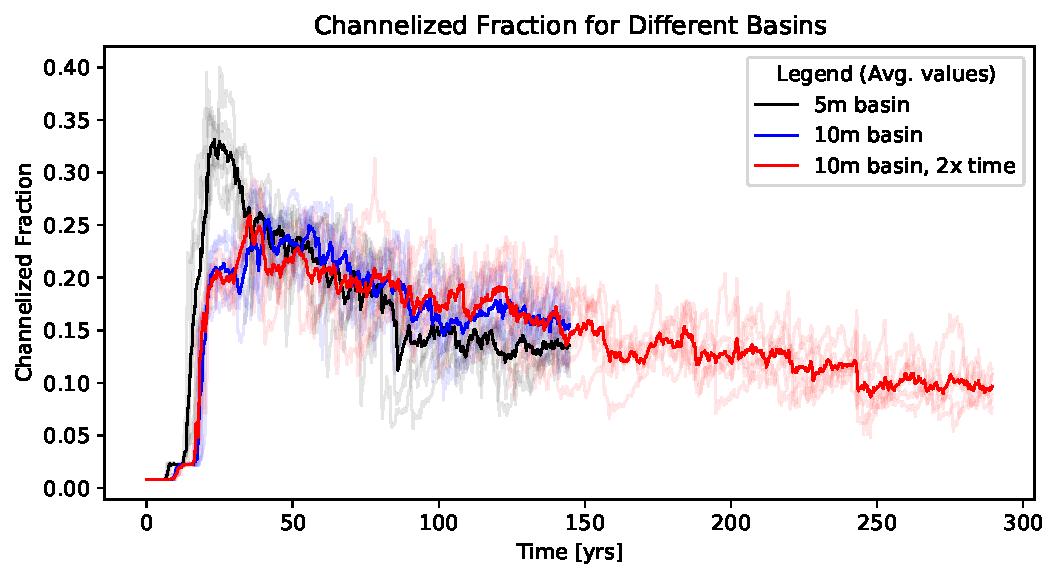
\includegraphics[width=\textwidth]{BasinDepth/figs/basin_chanfrac_timeseries.pdf}
	}	
	\caption{Timeseries of the fraction of the land area that is channelized.}
	\label{fig:bd_chanfrac_timeseries}
\end{figure}

\begin{figure}[!ht]
	\makebox[\textwidth][c]{
	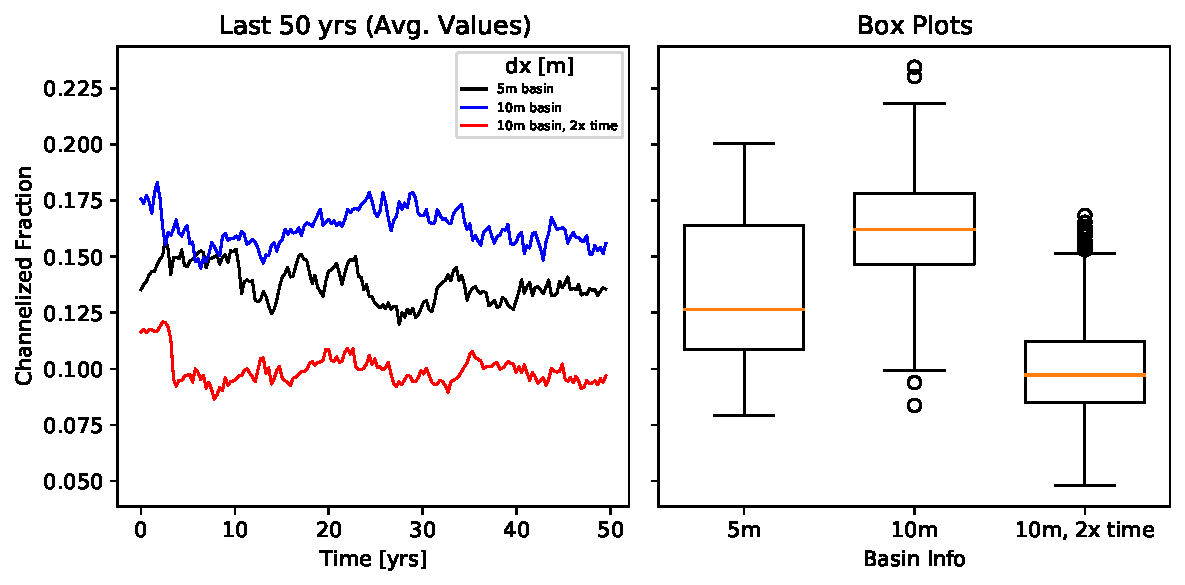
\includegraphics[width=\textwidth]{BasinDepth/figs/end_chanfrac_stationary.pdf}
	}	
	\caption{Average channel fraction from the final 50 years of each case (Left), and box plots of individual run channel fraction values over the final 50 years of each run split by basin scenario (Right).}
	\label{fig:bd_chanfrac_box}
\end{figure}

\begin{figure}[!ht]
	\makebox[\textwidth][c]{
	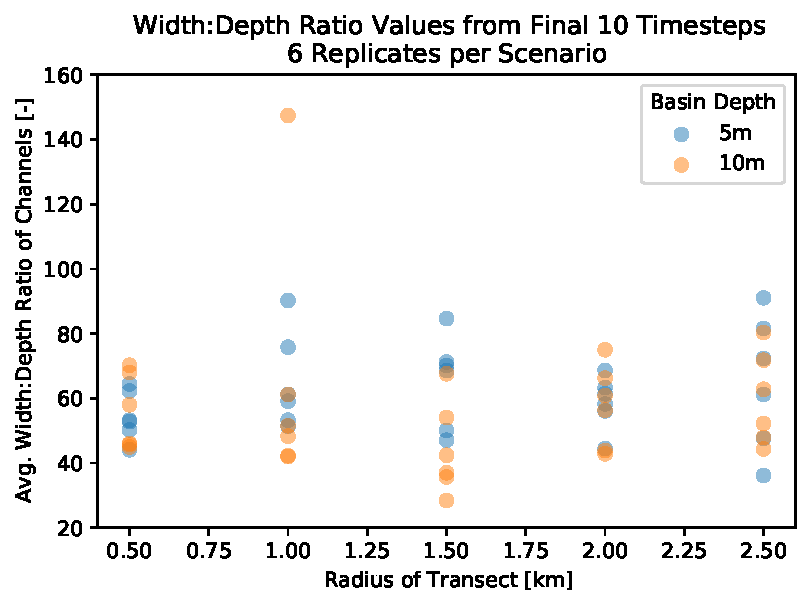
\includegraphics[width=\textwidth]{BasinDepth/figs/widthdepths_both.pdf}
	}	
	\caption{Average width-to-depth ratios from channels picked out along radial transects with different radii using the final 10 timesteps of the 5m deep basin scenario, and the 10m basin depth, 10,000 timestep scenario.}
	\label{fig:bd_wd}
\end{figure}

\section{Conclusions}
Beyond slowing the lateral growth of the system due to the deeper basin, there don't appear to be real differences between the two.
Both the width-to-depth ratios of the surface channels and the proportion of the subaerial surface that was channelized appeared to be similar (Figures \ref{fig:bd_wd} \& \ref{fig:bd_chanfrac_timeseries}).
When qualitatively looking at the stratigraphy, there is not much to comment on besides the obvious preservation of $\sim$ 10m of stratigraphy in the 10m basin, and $\sim$ 5m in the shallower 5m basin.

\clearpage
\bibliographystyle{plainnat}
\bibliography{bib/bib}